%%%%%%%%%%%%%%%%%%%%%%%%%%%%%%%%%%%%%%%%%%%%%%%%%%%%%%%%%%%%%%%%%%%%%%%%%%%%%%%%
\documentclass[12pt,conference]{ieeeconf} %Github
%\documentclass[letterpaper, 12 pt, onecolumn]{ieeeconf} %Prof. Parallel

% Comment this line out
                                                          % if you need a4paper
%\documentclass[a4paper, 10pt, conference]{ieeeconf}      % Use this line for a4
                                                          % paper

\IEEEoverridecommandlockouts                              % This command is only
                                                          % needed if you want to
                                                          % use the \thanks command
\overrideIEEEmargins
% See the \addtolength command later in the file to balance the column lengths
% on the last page of the document

% The following packages can be found on http:\\www.ctan.org
\usepackage{graphics} % for pdf, bitmapped graphics files
\usepackage{epsfig} % for postscript graphics files
%\usepackage{mathptmx} % assumes new font selection scheme installed
%\usepackage{times} % assumes new font selection scheme installed
\usepackage{amsmath} % assumes amsmath package installed
\usepackage{amssymb}  % assumes amsmath package installed

\usepackage{tikz}
\usetikzlibrary{shapes, arrows.meta, positioning}

\usepackage{url}
\usepackage[ruled, vlined, linesnumbered]{algorithm2e}
%\usepackage{algorithm}
\usepackage{verbatim} 
%\usepackage[noend]{algpseudocode}
\usepackage{soul, color}
\usepackage{lmodern}
\usepackage[hidelinks]{hyperref}
\usepackage{fancyhdr}
\usepackage[utf8]{inputenc}
\usepackage{fourier} 
\usepackage{array}
\usepackage{subcaption}
\usepackage{graphicx}
\usepackage{pgf}
\usepackage{makecell}
\usepackage[sorting=none]{biblatex} % For biblatex
\addbibresource{reference.bib} % Path to your .bib file

\SetNlSty{large}{}{:}

\renewcommand\theadalign{bc}
\renewcommand\theadfont{\bfseries}
\renewcommand\theadgape{\Gape[4pt]}
\renewcommand\cellgape{\Gape[4pt]}

\newcommand{\rework}[1]{\todo[color=yellow,inline]{#1}}

\makeatletter
\newcommand{\rom}[1]{\romannumeral #1}
\newcommand{\Rom}[1]{\expandafter\@slowromancap\romannumeral #1@}
\makeatother

\pagestyle{plain} 

\title{GATTO: Can Topological Information Improve Node Classification via GAT?\\
\large Final Report for Learning from Network's project \\}

\author{Francesco Biscaccia Carrara \textit{(2120934)}, Riccardo Modolo \textit{(2123750)},\\ Alessandro Viespoli \textit{(2120824)} % <-this % stops a space 
\\\\ Master Degree in Computer Engineering \\
University of Padova \\
}

\begin{document}

\maketitle
\thispagestyle{plain}
\pagestyle{plain}

%%%%%%%%%%%%%%%%%%%%%%%%%%%%%%%%%%%%%%%%%%%%%%%%%%%%%%%%%%%%%%%%%%%%%%%%%%%%%%%%
\begin{abstract}
    This study introduces GATTO (Graph Attention Network with TOpological Information), a framework designed to enhance the performance of Graph Attention Networks (GAT) for node classification tasks by incorporating topological features. The research evaluates GATTO on two citation network datasets (Cora and Citeseer) by adding four topological features. While GATTO showed slight improvements in absolute performance (0.14\%-0.54\%), statistical analysis revealed no significant difference compared to standard GAT implementation. The results indicate that the additional computational cost of the topological features does not justify their inclusion for small datasets.
\end{abstract}


%%%%%%%%%%%%%%%%%%%%%%%%%%%%%%%%%%%%%%%%%%%%%%%%%%%%%%%%%%%%%%%%%%%%%%%%%%%%%%%%
\section{Introduction} 
Node classification is a crucial research topic in graph-based learning and has significant applications in various fields, including social network analysis, recommendation systems, and biological networks. One of the most recent techniques for obtaining a high-quality node classifier is the Graph Attention Network (GAT), in which the graph's embedding is learned by considering the embeddings of neighboring nodes, scaled by learnable attention weights. By performing a transductive learning task, GAT achieves good generalization performance. However, we propose a new framework, GATTO (Graph Attention Network with TOpological Information), which aims to improve classic GAT classification by incorporating topological features derived from the graph or its embedding.

%%%%%%%%%%%%%%%%%%%%%%%%%%%%%%%%%%%%%%%%%%%%%%%%%%%%%%%%%%%%%%%%%%%%%%%%%%%%%%%%
\section{Data} 
\subsection{Original Data}
The datasets used are the same as those in the GAT$^\text{\cite{GAT}}$ paper. The table below summarizes the key characteristics of the datasets.
\begin{table}[h!] 
    \centering 
    \renewcommand{\arraystretch}{1.5} 
    \begin{tabular}{|l|c|c|c|c|} 
        \hline 
        \textbf{Network} & \textbf{Nodes} & \textbf{Edges} & \textbf{Labels} & \textbf{Features} \\
        \hline 
        Cora & 2708 & 5429 & 7 & 1443 \\
        Citeseer & 3327 & 4732 & 6 & 3703 \\
        \hline 
    \end{tabular} 
\end{table}
\\
In both datasets, each node has a single label. The graphs are directed, unweighted, and do not contain self-loops.

\subsection{Enhanced Data}
For our experiment, the following features are computed and assigned to each node:
\begin{itemize}
    \item \textbf{Degree Centrality}: The fraction of nodes to which a node is connected.
    \item \textbf{Betweenness Centrality}: The sum of the fractions of all-pairs shortest paths that pass through a given node.
    \item \textbf{Closeness Centrality}: The reciprocal of the average shortest path distance from a given node to all other reachable nodes.
    \item \textbf{Suggested Label}: The label assigned by clustering the graph's node embeddings.
\end{itemize}

%%%%%%%%%%%%%%%%%%%%%%%%%%%%%%%%%%%%%%%%%%%%%%%%%%%%%%%%%%%%%%%%%%%%%%%%%%%%%%%%
\section{Implementation} 
\subsection{Module Framework Idea}
The practical implementation$^{\text{\cite{GATTO}}}$ adheres to the conceptual framework. It consists of two main blocks:
\begin{itemize}
    \item \textbf{Precomputation Module}: The class that computes the extra features from the graph (or its embedding) and returns them as a feature matrix.
    \item \textbf{GAT Module}: The GAT implementation for training and predicting node labels.
\end{itemize}
The implementation of this framework is available on the GitHub repository in the \textit{code} section, written in Python 3.8.10 with the required packages listed in the Singularity.def file.
\subsection{Precomputation Module}
Topological features can be computed by importing the dataset into a NetworkX$^{\text{\cite{SciPyProceedings_11}}}$ object and using the available methods to calculate the desired features. For the embeddings, we use Node2Vec$^\text{\cite{node2vec}}$ with standard parameters. The resulting embeddings reside in $\mathbb{R}^{128}$, and based on the number of labels in the graph, we select:
\begin{itemize}
    \item \textbf{K-Means++} if $\log_{10}{(\text{labels})} < 2$.
    \item \textbf{AgglomerativeClustering} otherwise.
\end{itemize}
These clustering methods are implemented using the Scikit-learn package.
Since the framework is designed to be scalable and modular, the extra features are saved into a pandas DataFrame after the feature-building phase. This allows GATTO to function as a standard GAT network if the Precomputation step is skipped.

\subsection{GAT Module}
For our experiment, we use the same configuration presented in the GAT paper for \textbf{Transductive Learning}. \\
The network consists of a two-layer GAT model. 
\begin{enumerate}
    \item The first layer has $K = 8$ attention heads, each computing $F' = 8$ features, followed by an ELU (Exponential Linear Unit) activation.
    \item The second layer is used for classification: a single attention head computes $C$ features (where $C$ is the number of classes), followed by a softmax activation.
\end{enumerate}
A dropout rate of $p = 0.5$ is applied to both the layers' inputs and the \textit{normalized attention coefficients}.\\
For the loss function, we use \textit{cross-entropy loss}. \\This is implemented using the TensorFlow and StellarGraph packages.
Since the input data to the GAT model is binary, we \textit{binarize} the data before training.

%%%%%%%%%%%%%%%%%%%%%%%%%%%%%%%%%%%%%%%%%%%%%%%%%%%%%%%%%%%%%%%%%%%%%%%%%%%%%%%%
\section{Performance Analysis} 
\subsection{Experimental Setup}
The algorithms were executed on two different machines: the \textit{CAPRI High-Performance Computing} system for feature matrix extraction and a general-purpose computer equipped with an \textit{Nvidia RTX 2060} GPU for training and tuning the GAT network. The dataset was divided such that $70\%$ was allocated for training, $10\%$ of the remaining $30\%$ was used for validation, and the rest was reserved for testing.

\subsection{Statistical Test}
To compare the performance of the GATTO algorithm with the GAT baseline algorithm, we conducted $10$ runs for each technique on each dataset. The following parameters were estimated during the evaluation:
\begin{itemize} 
    \item \textbf{Accuracy}: The ratio of correctly predicted instances to the total number of instances. 
    \item \textbf{Precision}: The ratio of true positive predictions to the total number of positive predictions. 
    \item \textbf{Recall}: The ratio of true positive predictions to the total number of actual positive instances. 
    \item \textbf{F1 Score}: The harmonic mean of precision and recall, providing a balanced measure of the two. 
\end{itemize}
We employ the following statistical tests to evaluate and compare the performance of the algorithms:
\begin{enumerate} 
    \item Since all scores are bounded in $[0,1]$, we use the Shapiro-Wilk Test to assess the normality of the score distributions. 
    \item If the Shapiro-Wilk Test indicates normality, we perform: 
        \begin{itemize} 
            \item Two-Sample t-Test under the assumption of equal variances. 
            \item Two-Sample t-Test under the assumption of unequal variances. 
            \item Wilcoxon Signed-Rank Test as a non-parametric alternative. 
        \end{itemize} 
        \item If the Shapiro-Wilk Test rejects normality, we rely solely on the Wilcoxon Signed-Rank Test, as this provides robust results in non-normal scenarios. 
\end{enumerate}
The described statistical tests are implemented and available in the GitHub repository as the \textit{Results.R} file, located in the \textit{code/results} section.

%%%%%%%%%%%%%%%%%%%%%%%%%%%%%%%%%%%%%%%%%%%%%%%%%%%%%%%%%%%%%%%%%%%%%%%%%%%%%%%%
\section{Results} 
The following tables present the mean and variance of each score for each algorithm, computed based on the previously described tests.
\begin{table}[h!]
    \centering
    \begin{tabular}{|l|c|c|c|c|} 
    \hline
     & Accuracy & Precision & Recall & F1 Score \\ \hline
    GAT &$0.888$ &$0.891$ &$0.888$ &$0.888$ \\ \hline
    GATTO &$0.890$ &$0.893$ &$0.890$ &$0.890$\\ \hline
    \end{tabular}
    \caption{{Cora}: Averages of the scores for GAT and GATTO}
\end{table}

\begin{table}[h!]
    \centering 
    \begin{tabular}{|l|c|c|c|c|} 
    \hline
     & Accuracy & Precision & Recall & F1 Score \\ \hline
    GAT &$2.566\text{e}-5$ &$2.693\text{e}-5$ &$2.566\text{e}-5$ &$2.564\text{e}-5$ \\ \hline
    GATTO &$1.823\text{e}-5$ &$1.611\text{e}-5$ &$1.823\text{e}-5$ &$1.837\text{e}-5$\\ \hline
    \end{tabular}
    \caption{\textbf{Cora}: Variances of the scores for GAT and GATTO}
\end{table}

\begin{table}[h!]
    \centering
    \begin{tabular}{|l|c|c|c|c|} 
    \hline
     & Accuracy & Precision & Recall & F1 Score \\ \hline
    GAT &$0.737$ &$0.732$ &$0.737$ &$0.731$ \\ \hline
    GATTO &$0.736$ &$0.731$ &$0.736$ &$ 0.730$\\ \hline
    \end{tabular}
    \caption{\textbf{CiteSeer}: Averages of the scores for GAT and GATTO}
\end{table}

\begin{table}[h!]
    \centering 
    \begin{tabular}{|l|c|c|c|c|} 
    \hline
     & Accuracy & Precision & Recall & F1 Score \\ \hline
    GAT &$2.580\text{e}-5$ &$2.819\text{e}-5$ &$2.580\text{e}-5$ &$2.911\text{e}-5$ \\ \hline
    GATTO &$1.011\text{e}-5$ &$9.231\text{e}-6$ &$1.011\text{e}-5$ &$9.936\text{e}-6$\\ \hline
    \end{tabular}
    \caption{\textbf{CiteSeer}: Variances of the scores for GAT and GATTO}
\end{table}
From a superficial analysis, it appears that GATTO performs slightly better in terms of both average and variance values. However, after running the statistical tests described in the previous section [Table \ref{table:Cora_Pval} and Table \ref{table:CiteSeer_Pval}], we find that, under the condition of a Type-I error bound $\alpha \leq 0.05$, the p-values returned by the tests indicate there is no statistically significant evidence that the algorithms perform differently, at least on small datasets.

This result might be attributed to the minimal impact of adding a small "piece of information" to the nodes (4 features out of 1447 for Cora, and 4 features out of 3707 for CiteSeer), which does not significantly influence the overall performance of the GAT network. Based on these considerations, the Precomputation Module can be discarded, as it is computationally expensive and does not yield a meaningful performance improvement. While it provides a modest absolute boost of $0.14\%-0.54\%$, this improvement is not substantial enough to justify the additional computational cost.

\subsection{Confusion Matrices}
For each run, the corresponding confusion matrix was saved. All plots are available in the \textit{code/logs} section, with a selection provided as examples [Figure \ref{fig:Confusion_Matrices}].
\begin{table*}[h!]
    \centering 
    \begin{tabular}{|l|c|c|c|} 
    \hline
     & 2S-T-Test (same variance) & 2S-T-Test (diff variance) & Wilcoxon-Test\\ \hline
    Accuracy &$0.546$ &$0.546$ &$0.670$ \\ \hline
    Precision &$0.529$ &$0.530$ &$0.570$\\ \hline
    Recall &$0.546$ &$0.546$ &$0.670$\\ \hline
    F1 Score &$0.524$ &$0.525$ &$0.677$\\ \hline
    \end{tabular}
    \caption{\textbf{Cora}: P-values for each test}
    \label{table:Cora_Pval}
\end{table*}

\begin{table*}[h!]
    \centering 
    \begin{tabular}{|l|c|c|c|} 
    \hline
     & 2S-T-Test (same variance) & 2S-T-Test (diff variance) & Wilcoxon-Test\\ \hline
    Accuracy &/ &/ &$0.908$ \\ \hline
    Precision &$0.567$ &$0.569$ &$0.969$\\ \hline
    Recall &/ &/ &$0.908$\\ \hline
    F1 Score &$0.583$ &$0.585$ &$0.969$\\ \hline
    \end{tabular}
    \caption{\textbf{CiteSeer}: P-values for each test}
    \label{table:CiteSeer_Pval}
\end{table*}

\begin{figure*}[h!]
    \begin{subfigure}[t]{.4\textwidth}
      \centering
      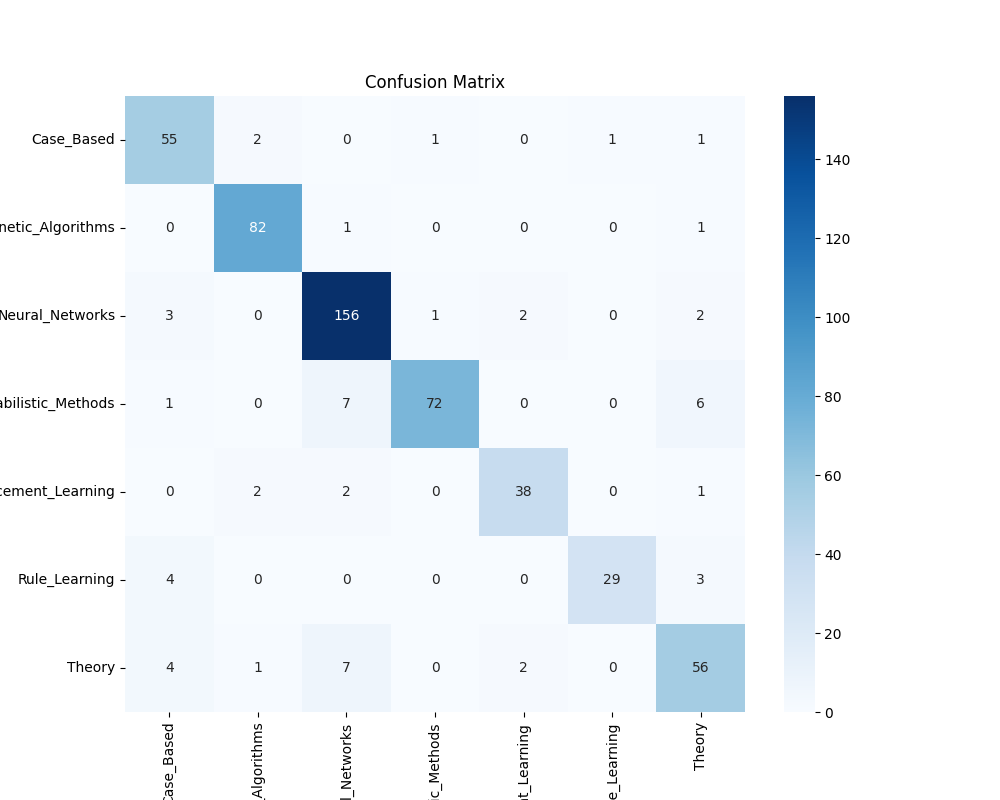
\includegraphics[width=\linewidth]{img/Cora_CM_GAT.png}
      \caption{\textbf{Cora}: confusion matrix without additional features}
    \end{subfigure}
    \hfill
    \begin{subfigure}[t]{.4\textwidth}
      \centering
      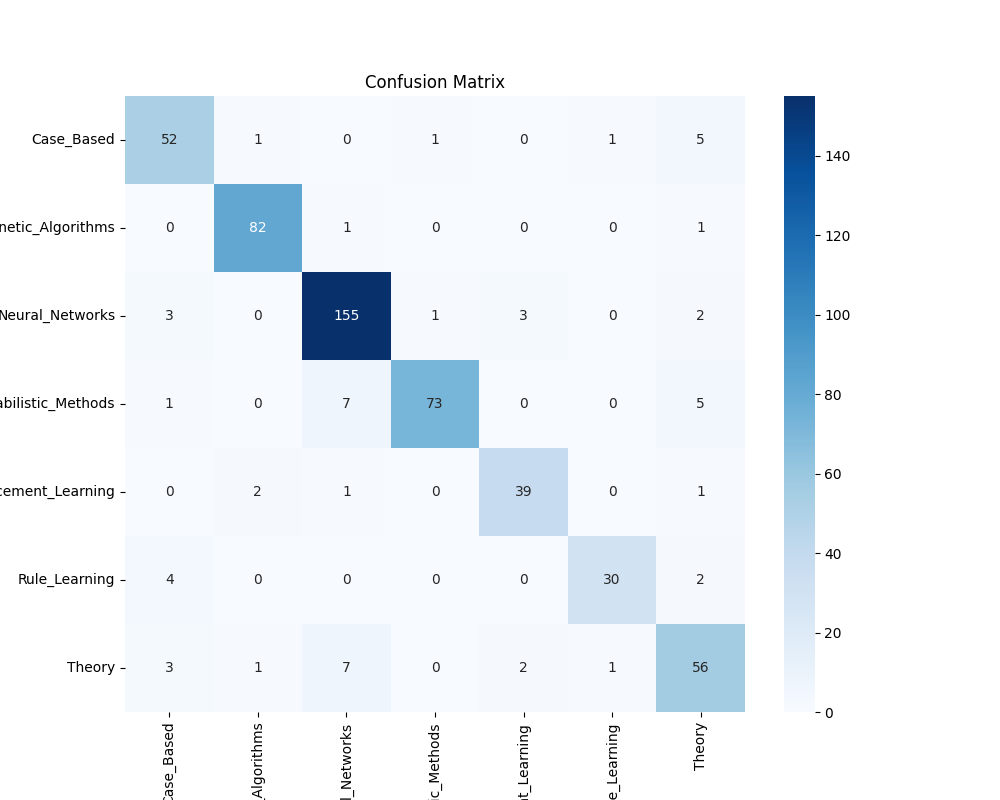
\includegraphics[width=\linewidth]{img/Cora_CM_GATTO.png}
      \caption{\textbf{Cora}: Confusion Matrix with additional features}
    \end{subfigure}
  
    \medskip
  
    \begin{subfigure}[t]{.4\textwidth}
      \centering
      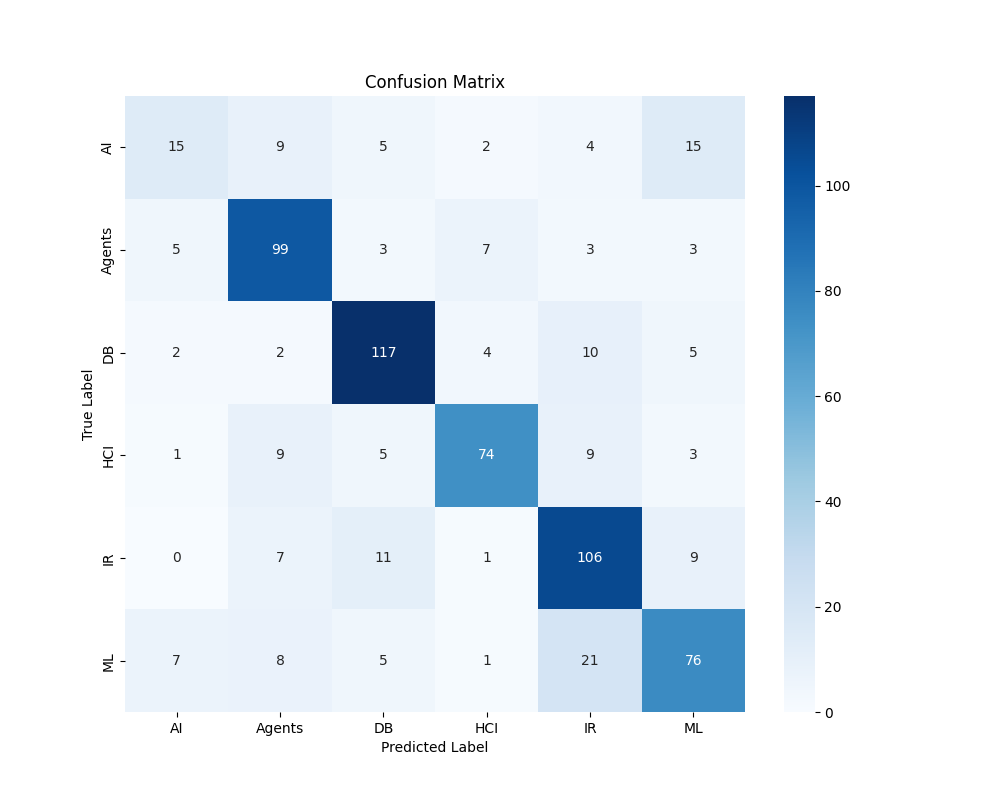
\includegraphics[width=\linewidth]{img/CiteSeer_CM_GAT.png}
      \caption{\textbf{CiteSeer}: Confusion Matrix without additional features}
    \end{subfigure}
    \hfill
    \begin{subfigure}[t]{.4\textwidth}
      \centering
      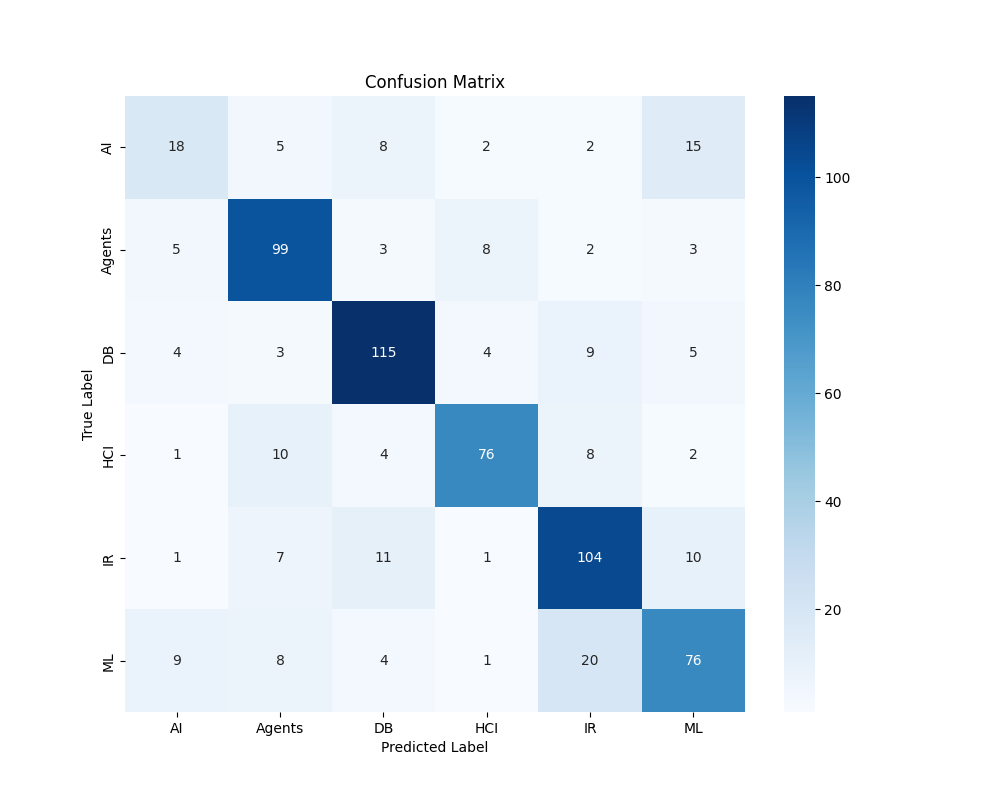
\includegraphics[width=\linewidth]{img/CiteSeer_CM_GATTO.png}
      \caption{\textbf{CiteSeer}: Confusion Matrix with additional features}
    \end{subfigure}
    \caption{Confusion Matrices for GAT and GATTO}
    \label{fig:Confusion_Matrices}
  \end{figure*}

%%%%%%%%%%%%%%%%%%%%%%%%%%%%%%%%%%%%%%%%%%%%%%%%%%%%%%%%%%%%%%%%%%%%%%%%%%%%%%%%
\section{Conclusion and Future works}
As discussed in the previous section, in terms of performance and efficiency, the Precomputation Module can be omitted, relying solely on the GAT module.\\
However, several potential improvements could be explored in future work:
\begin{enumerate}
\item Experiment with different types of embeddings prior to the clustering phase.
\item Explore alternative clustering techniques, potentially leveraging MapReduce for scalability.
\item Evaluate GATTO on larger datasets to test its scalability and effectiveness.
\item Perform extensive hyperparameter tuning for the GAT module to optimize performance.
\item Extend the GATTO model to graphs with nodes lacking native features.
\end{enumerate}



%%%%%%%%%%%%%%%%%%%%%%%%%%%%%%%%%%%%%%%%%%%%%%%%%%%%%%%%%%%%%%%%%%%%%%%%%%%%%%%%
\vspace{\fill}
\section*{Work Report}
In this section, we describe the distribution of the work and the detailed contributions of each member.
\begin{itemize}
    \item \textit{Francesco Biscaccia Carrara (2120934)}: {\textbf{40\% of the work}. Developed the code for the Precomputation Module, ran tests on CAPRI, and performed statistical tests.}
    \item \textit{Riccardo Modolo (2123750)}: {\textbf{40\% of the work}. Developed the code to retrieve data, reviewed the code, and wrote the Proposal, Midterm, and Final Paper.}
    \item \textit{Alessandro Viespoli (2120824)}: {\textbf{20\% of the work}. Developed the code for the GAT model and for plotting the results.}
    \item \textit{ChatGPT}: {Contributed to correcting grammar errors and producing the tables.}
\end{itemize}
\printbibliography
\newpage

%%%%%%%%%%%%%%%%%%%%%%%%%%%%%%%%%%%%%%%%%%%%%%%%%%%%%%%%%%%%%%%%%%%%%%%%%%%%%%%%
\end{document}